\documentclass[conference]{IEEEtran}
\IEEEoverridecommandlockouts
\usepackage{cite}
\usepackage{amsmath,amssymb,amsfonts}
\usepackage{algorithmic}
\usepackage{graphicx}
\usepackage{textcomp}
\usepackage{xcolor}
\usepackage{booktabs}
\usepackage{tikz}
\usetikzlibrary{arrows.meta,positioning,shapes.geometric,calc,fit,backgrounds}
\usepackage[hidelinks]{hyperref}
\usepackage{url}
\usepackage{multirow}
\usepackage{listings}

\lstdefinestyle{shellbox}{
  basicstyle=\ttfamily\scriptsize,
  breaklines=true,
  breakatwhitespace=true,
  showstringspaces=false,
  columns=fullflexible,
  keepspaces=true,
  xleftmargin=2pt,
  xrightmargin=2pt,
  frame=single,
  framerule=0.3pt,
  rulecolor=\color{black!40},
  backgroundcolor=\color{black!4},
  prebreak=\mbox{\tiny$\hookleftarrow$},
  language=bash
}

\def\BibTeX{{\rm B\kern-.05em{\sc i\kern-.025em b}\kern-.08em
    T\kern-.1667em\lower.7ex\hbox{E}\kern-.125emX}}

\begin{document}

\title{Two-Tier Pre-Execution Defense Against\\Type-C Command-Path Attacks in Smart-Grid SCADA}

\author{\IEEEauthorblockN{Sungyoun Seo}
\IEEEauthorblockA{\textit{Department of Electrical and Computer Engineering} \\
\textit{University of Rhode Island}\\
Kingston, RI, USA}
}

\maketitle

\begin{abstract}
Type-C command-path attacks substitute a physically unsafe setpoint inside a protocol-conformant control packet, bypassing signature-based intrusion detection. We implement and evaluate a relay-side two-tier defense: a tier-1 nominal-band check followed by a tier-2 linearized DC consequence score derived from the IEEE 9-bus measurement Jacobian. A controlled stealthy-attack ablation on a Mininet testbed reveals the distinct role of each tier: tier-2 alone provides the correctness guarantee, blocking both gross and stealthy attacks, while tier-1 acts as a fast pre-filter that short-circuits the physics evaluation for easily-detectable out-of-band commands, reducing latency $7\times$ (0.357~ms $\to$ 0.052~ms) for gross attacks. Tier-1 alone, however, misses in-band rewrites that tier-2 catches via the DC consequence score.
\end{abstract}

\begin{IEEEkeywords}
cyber-physical security, smart grid, false data injection, command injection, intrusion detection, Mininet
\end{IEEEkeywords}

\section{Introduction}\label{sec:intro}
Wide-area power-grid SCADA networks rely on lightweight protocols such as DNP3 \cite{dnp3spec} that authenticate packet structure but not packet \emph{intent}. Liu \emph{et al.}\ \cite{liuFalseDataInjection} showed that an attacker controlling a subset of meters can inject coordinated false measurements that pass weighted-least-squares residual checks (\emph{Type-A} read-path attack). Lin \emph{et al.}\ \cite{linSafetycriticalCyberphysicalAttacks2016,linChallengesOpportunitiesDetection2020} define \emph{Type-C} attacks on the \emph{write} path: a MitM node intercepts a control command and substitutes a physically dangerous yet protocol-conformant setpoint. Signature- and specification-based IDS \cite{aliConfigurationbasedIDSAdvanced2013,senSpecificationbasedCyberattackDetection2022,yangMultiattributeSCADA2014} cannot distinguish the malicious value from a benign one without modeling the underlying physics.

A hard nominal band catches gross attacks but is blind to a sophisticated attacker who stays inside the band. Existing defenses such as moving-target control \cite{kanellopoulosMovingTargetDefense2020}, reachability analysis \cite{zhangReachabilityAnalysisCyberPhysical2022}, and process-aware IDS \cite{menzelRealworldCaseStudies2025} operate post-execution; \cite{linSafetycriticalCyberphysicalAttacks2016} instead proposes consequence reasoning at the relay \emph{before} state is updated. We implement that principle as two stacked checks and use a Mininet stealthy-attack ablation to quantify each tier's marginal contribution.

\textbf{Contributions.} (i) A Mininet harness \cite{lantzMininet2010,zhuSCADATaxonomy2011} with a MitM aggregator mounting Type-A FDIA and Type-C rewrites; (ii) a relay-side defense combining a nominal band and a linearized DC consequence score; (iii) a controlled ablation that isolates the distinct role of each tier: tier-2 provides the security guarantee while tier-1 serves as a latency-reducing pre-filter, together achieving both correctness and efficiency.

\section{Threat Model and System Design}\label{sec:design}
\subsection{Network and Protocol}
The emulated topology (Fig.~\ref{fig:topo}) uses Mininet \cite{lantzMininet2010} with three Open vSwitch switches, one control center (\texttt{cc}), one data aggregator (\texttt{da}) acting as the MitM vantage point, and four protection relays. The control center exchanges a binary DNP3-like protocol (DNP3m) with \texttt{da} on TCP port 20000; \texttt{da} relays messages downstream to each relay on separate sockets. Three opcodes suffice: poll (\texttt{0x01}), control (\texttt{0x02}, 7-byte index + setpoint), and ack (\texttt{0x0C}, status accept/reject).

\begin{figure}[t]
\centering
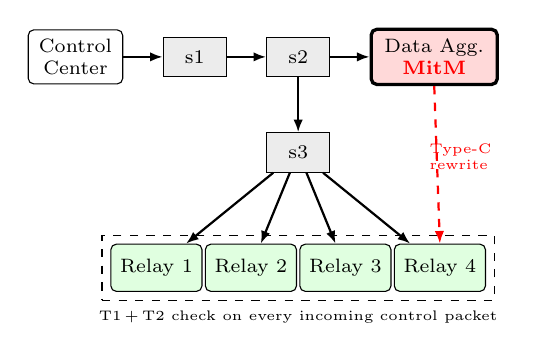
\begin{tikzpicture}[
  font=\scriptsize,
  node/.style={draw, rounded corners=2pt, minimum width=12mm, minimum height=6mm, align=center},
  sw/.style={draw, fill=gray!15, minimum width=8mm, minimum height=5mm},
  mitm/.style={draw, fill=red!15, rounded corners=2pt, minimum width=16mm, minimum height=7mm, align=center, very thick},
  relay/.style={draw, fill=green!12, rounded corners=2pt, minimum width=10mm, minimum height=6mm, align=center},
  arr/.style={-{Latex[length=1.6mm]}, thick}
]
  \node[node] (cc) {Control\\Center};
  \node[sw, right=5mm of cc] (s1) {s1};
  \node[sw, right=5mm of s1] (s2) {s2};
  \node[mitm, right=5mm of s2] (da) {Data Agg.\\{\textcolor{red}{\textbf{MitM}}}};
  \node[sw, below=7mm of s2] (s3) {s3};
  \node[relay, below=9mm of s3, xshift=-18mm] (r1) {Relay 1};
  \node[relay, below=9mm of s3, xshift=-6mm]  (r2) {Relay 2};
  \node[relay, below=9mm of s3, xshift= 6mm]  (r3) {Relay 3};
  \node[relay, below=9mm of s3, xshift= 18mm] (r4) {Relay 4};

  % Dashed box around relays with T1+T2 label
  \node[draw, dashed, inner sep=3pt,
        fit=(r1)(r2)(r3)(r4),
        label={[font=\tiny]below:{T1\,+\,T2 check on every incoming control packet}}] (rbox) {};

  \draw[arr] (cc) -- (s1);
  \draw[arr] (s1) -- (s2);
  \draw[arr] (s2) -- (da);
  \draw[arr] (s2) -- (s3);
  \draw[arr] (s3) -- (r1);
  \draw[arr] (s3) -- (r2);
  \draw[arr] (s3) -- (r3);
  \draw[arr] (s3) -- (r4);

  % Type-C attack: da rewrites setpoint and injects directly into relays
  \draw[red, dashed, -{Latex[length=1.6mm]}, thick]
    (da.south) -- (r4.north);
  \node[red, font=\tiny, align=left] at ($(da.south)!0.45!(r4.north)+(3mm,0)$)
    {Type-C\\rewrite};
\end{tikzpicture}
\caption{Mininet topology. \texttt{da} sits between the control center and the four relays. With \texttt{TYPE\_C\_ATTACK} enabled, it rewrites the operator's setpoint before forwarding (red dashed path). Every relay applies the tier-1 + tier-2 check on the incoming packet \emph{before} updating local state.}
\label{fig:topo}
\end{figure}

\subsection{Attack Model}
The data aggregator implements both attack classes as toggleable behaviours:
\begin{itemize}
\item \textbf{Type-A (FDIA).} On every poll the aggregator overwrites the relay-supplied measurement vector with a precomputed FDIA mapping $\bar{\mathbf{z}}$ chosen following \cite{liuFalseDataInjection}.
\item \textbf{Type-C (MitM rewrite).} For every \texttt{0x02} control packet the aggregator replaces the originally requested setpoint with a malicious value $\mathrm{sp}_{\mathrm{atk}}$ and forwards the otherwise-identical frame downstream. We test both a \emph{gross} attack ($\mathrm{sp}_{\mathrm{atk}}=8.0$~pu, far outside any nominal band) and a \emph{stealthy} attack ($\mathrm{sp}_{\mathrm{atk}}=2.5$~pu, inside the tier-1 band but with a non-trivial physical effect).
\end{itemize}
The four operational modes are the cross-product of the two toggles: \texttt{baseline}, \texttt{fdia\_only}, \texttt{typec\_only}, and \texttt{combined}.

\section{Relay-Side Two-Tier Defense}\label{sec:defense}
The defense executes inside the relay process when a control packet arrives, before any local state update. Fig.~\ref{fig:flow} summarizes the decision path.

\subsection{Tier-1: Nominal Operating Band}
Each relay holds a table of nominal real-power injection setpoints $z_{\mathrm{nom}}[k]$ for the indices it owns (e.g.\ index $23\!\to\!1.63$~pu). Tier-1 rejects any setpoint outside the symmetric envelope
\begin{equation}
\bigl|\mathrm{sp} - z_{\mathrm{nom}}[k]\bigr| \le \Delta_{\max}, \quad \Delta_{\max}=1.0~\text{pu}.
\label{eq:tier1}
\end{equation}
The gross malicious value 8.0~pu fails (\ref{eq:tier1}) for every defined index and is rejected with reason \texttt{tier1\_band\_violation}. Tier-1 alone, however, cannot distinguish a stealthy in-band attack from a legitimate command. Its role in the combined defense is therefore that of a \emph{latency-reducing pre-filter}: it short-circuits the more expensive tier-2 evaluation for commands that are trivially out-of-band, while passing all in-band commands to tier-2 for physics-based scrutiny.

\subsection{Tier-2: Linearized DC Consequence Score}
Tier-2 evaluates the predicted physical effect of an admissible command using the DC measurement model from \texttt{calculate\_fdia.m}. Let $\mathbf{H}\in\mathbb{R}^{9\times8}$ be the measurement Jacobian of the IEEE 9-bus topology, $\mathbf{W}=100\mathbf{I}$ the WLS weight, and
\begin{equation}
\mathbf{G} = (\mathbf{H}^{\top}\mathbf{W}\mathbf{H})^{-1}\mathbf{H}^{\top}\mathbf{W}.
\label{eq:gain}
\end{equation}
For a proposed setpoint $\mathrm{sp}$ at injection index $k$, the relay constructs $\Delta\mathbf{z}\in\mathbb{R}^{9}$ with $\Delta z_k = \mathrm{sp}-z_{\mathrm{nom}}[k]$ (other components zero) and computes the consequence severity
\begin{equation}
s = \bigl\lVert \mathbf{G}\,\Delta\mathbf{z}\bigr\rVert_{\infty}.
\label{eq:sev}
\end{equation}
The command is rejected if $s>\tau$, with $\tau=0.10$~pu calibrated on the 9-bus model. Fig.~\ref{fig:sev} shows $s$ vs.\ setpoint at index 23: severity crosses $\tau$ at sp$\approx 2.35$~pu---still inside the tier-1 band---carving a tighter safe sub-region where a sophisticated attacker would operate. $\mathbf{G}$ is cached at startup; each subsequent evaluation is a single $9{\to}8$ matrix--vector multiply.

\begin{figure}[t]
\centering
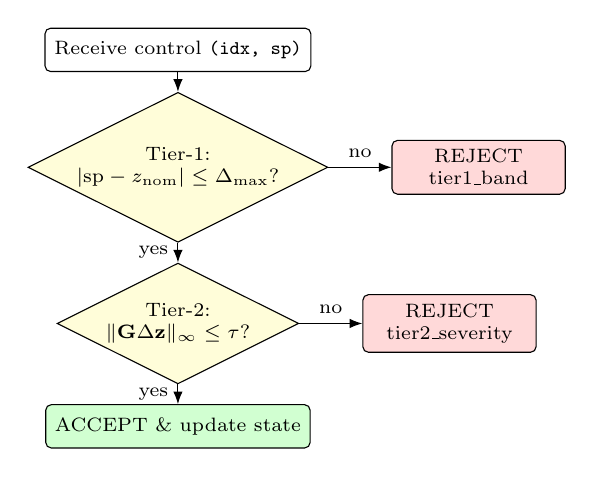
\begin{tikzpicture}[
  font=\scriptsize, node distance=2.5mm,
  proc/.style={draw, rounded corners=2pt, minimum width=22mm, minimum height=5.5mm, align=center},
  dec/.style={draw, diamond, aspect=2.0, inner sep=1pt, align=center, fill=yellow!15},
  bad/.style={draw, rounded corners=2pt, fill=red!15, minimum width=22mm, minimum height=5.5mm, align=center},
  good/.style={draw, rounded corners=2pt, fill=green!18, minimum width=22mm, minimum height=5.5mm, align=center},
  arr/.style={-{Latex[length=1.6mm]}}
]
  \node[proc] (rcv) {Receive control \texttt{(idx, sp)}};
  \node[dec, below=of rcv] (t1) {Tier-1:\\$|\mathrm{sp}-z_\mathrm{nom}|\le\Delta_{\max}$?};
  \node[bad, right=8mm of t1] (rej1) {REJECT\\\scriptsize tier1\_band};
  \node[dec, below=of t1] (t2) {Tier-2:\\$\lVert\mathbf{G}\Delta\mathbf{z}\rVert_\infty\le\tau$?};
  \node[bad, right=8mm of t2] (rej2) {REJECT\\\scriptsize tier2\_severity};
  \node[good, below=of t2] (acc) {ACCEPT \& update state};

  \draw[arr] (rcv) -- (t1);
  \draw[arr] (t1) -- node[left]{yes} (t2);
  \draw[arr] (t1) -- node[above]{no} (rej1);
  \draw[arr] (t2) -- node[left]{yes} (acc);
  \draw[arr] (t2) -- node[above]{no} (rej2);
\end{tikzpicture}
\caption{Relay-side decision flow. Tier-1 fast-rejects gross band violations; tier-2 evaluates the linearized DC severity for in-band commands.}
\label{fig:flow}
\end{figure}

\begin{figure}[t]
\centering
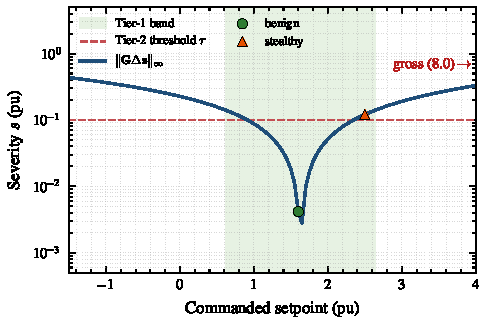
\includegraphics[width=0.95\columnwidth]{figures/fig_severity_sweep.pdf}
\caption{Tier-2 severity $s$ vs.\ setpoint (index 23). Green band: tier-1 region $[0.63,2.63]$~pu; red dashed: threshold $\tau\!=\!0.10$. Benign sp$=1.62$ sits at $s\!\approx\!10^{-3}$; stealthy sp$=2.50$ is inside the band but above $\tau$; gross sp$=8.0$ is outside both.}
\label{fig:sev}
\end{figure}

\section{Experimental Evaluation}\label{sec:results}
We report two experiments: a full Mininet matrix exercising the network stack, and a stealthy-attack ablation comparing tier configurations under an in-band MitM rewrite.

\subsection{Mininet Matrix Outcomes}
Four operational modes are swept across three setpoint profiles (Fig.~\ref{fig:mode}). \texttt{baseline} and \texttt{fdia\_only} are statistically indistinguishable, confirming that read-path corruption does \emph{not} affect the write-path defense. \texttt{typec\_only} and \texttt{combined} drop to a $22\%$ accept rate because the gross malicious value trips tier-1 on every event. Median latency is $\sim$0.05~ms in attack modes (tier-1 early exit) and $\sim$0.25~ms in benign modes (full tier-2 evaluation).

\begin{figure}[t]
\centering
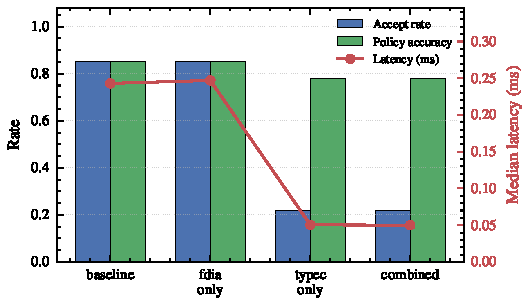
\includegraphics[width=0.95\columnwidth]{figures/fig_mode_results.pdf}
\caption{Per-mode accept rate, policy accuracy (left axis), and median relay latency (right axis). \texttt{fdia\_only} matches \texttt{baseline}; \texttt{typec\_only} matches \texttt{combined}.}
\label{fig:mode}
\end{figure}

Fig.~\ref{fig:confusion} reports the pooled $2\!\times\!2$ confusion outcome over all 328 events: 140 benign forwarded, 24 benign blocked, 36 attack forwarded, 128 attack blocked, for an overall policy accuracy of $0.817$. The 36 attack-forwarded and 24 benign-blocked events are entirely confined to ablation cells in which one or both tiers are intentionally disabled.

\begin{figure}[t]
\centering
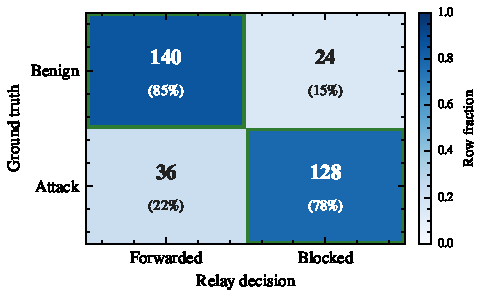
\includegraphics[width=0.85\columnwidth]{figures/fig_confusion.pdf}
\caption{Pooled confusion outcomes across all 328 paired control events. Cells display absolute counts and row fractions; green outline marks correct outcomes. All misses and false blocks come from ablation cells with deliberately disabled tiers.}
\label{fig:confusion}
\end{figure}

\subsection{Stealthy-Attack Ablation: Where Tier-2 is Decisive}
The matrix above uses a fixed gross setpoint (8.0~pu) that any band check defeats. To expose the in-band regime, we swept three scenarios under all four tier configurations: \emph{benign} (sp$=1.62$, no rewrite, $s\!=\!1.4\!\times\!10^{-3}$); \emph{stealthy} (MitM rewrites to 2.50~pu, inside tier-1 band, $s\!=\!0.121\!>\!\tau$); \emph{gross} (MitM rewrites to 8.00~pu, $s\!=\!0.884$).

Table~\ref{tab:stealthy} shows the full decision and latency breakdown (trials were unanimous). Three findings stand out. First, \emph{tier-2 alone blocks every attack}: both gross (REJ, 0.357~ms) and stealthy (REJ, 0.446~ms), making it the correctness guarantee of the design. Second, \emph{tier-1 alone is insufficient}: it accepts the stealthy in-band 2.5~pu rewrite because the value lies within the $\pm1.0$~pu band. Third, \emph{tier-1 serves as a latency pre-filter}: in the combined T1+T2 configuration, gross attacks are fast-rejected by tier-1 at 0.052~ms---a $6.9\times$ speedup over tier-2 alone (0.357~ms)---while stealthy attacks pass tier-1 and are correctly handled by tier-2. The benign command passes both tiers under all configurations, confirming zero false positives at the operator's true setpoint.

\begin{table}[t]
\caption{Relay Decision and Latency by Scenario and Defense Configuration}
\label{tab:stealthy}
\centering
\begin{tabular}{@{}llcccc@{}}
\toprule
\textbf{Scenario} & \textbf{sp} & \textbf{T1} & \textbf{T2} & \textbf{Decision} & \textbf{Lat.\ (ms)} \\
\midrule
\multirow{4}{*}{benign}
  & \multirow{4}{*}{1.62}
                & Y & Y & ACC        & 0.327 \\
  &             & Y & N & ACC        & 0.057 \\
  &             & N & Y & ACC        & 0.390 \\
  &             & N & N & ACC        & 0.048 \\
\midrule
\multirow{4}{*}{stealthy}
  & \multirow{4}{*}{2.50}
                & Y & Y & REJ              & 0.347 \\
  &             & Y & N & \textbf{ACC}$^*$ & 0.061 \\
  &             & N & Y & REJ              & 0.446 \\
  &             & N & N & \textbf{ACC}$^*$ & 0.045 \\
\midrule
\multirow{4}{*}{gross}
  & \multirow{4}{*}{8.00}
                & Y & Y & REJ              & 0.052 \\
  &             & Y & N & REJ              & 0.053 \\
  &             & N & Y & REJ              & 0.357 \\
  &             & N & N & \textbf{ACC}$^*$ & 0.044 \\
\bottomrule
\multicolumn{6}{@{}l@{}}{\footnotesize $^*$Wrong policy: attack not blocked.}
\end{tabular}
\end{table}

\subsection{Discussion}
Three properties hold across both experiments. \emph{Decoupling:} FDIA on the read path does not affect the write-path decision; the two attack surfaces are independent by construction, consistent with \cite{xiaoLimitsResidualBasedDetection2026}. \emph{Complementary tier roles:} tier-2 is the security-critical layer---it alone provides the correctness guarantee by evaluating physical consequence for every in-band command. Tier-1 is the efficiency layer---it cannot replace tier-2, but eliminates redundant tier-2 evaluations for trivially out-of-band commands, yielding a $6.9\times$ latency reduction on gross attacks. Deploying tier-1 without tier-2 sacrifices correctness; deploying tier-2 without tier-1 sacrifices efficiency but not safety. The optimal deployment is T1+T2: tier-1 filters, tier-2 decides. \emph{Cost:} even tier-2 alone completes in $<\!0.5$~ms, well below typical SCADA polling intervals; the combined defense further reduces this to $<\!0.06$~ms for the common case of gross out-of-band commands. The DC severity (\ref{eq:sev}) is a linearization calibrated on the 9-bus model; an AC or digital-twin extension \cite{senDigitalTwinEvaluating2023} would tighten discrimination at the cost of higher computation.

\subsection{How to Reproduce}
\begin{lstlisting}[style=shellbox]
pip install -r requirements.txt
sudo python3 run_experiment_matrix.py \
     --trials 3 --rounds 2 --skip-existing
python3 analyze_results.py
python3 report/figures/make_plots.py
\end{lstlisting}
\texttt{run\_experiment\_matrix.py} runs both the mode/profile matrix (Phase~1) and the stealthy-attack ablation (Phase~2) in sequence. Use \texttt{--skip-matrix} or \texttt{--skip-stealthy} to run either phase alone.

\section{Conclusion}\label{sec:conclusion}
A controlled stealthy-attack ablation on a Mininet nine-bus testbed reveals the complementary roles of a two-tier relay-side defense. Tier-2---a linearized DC consequence score---is the correctness-critical layer: it alone blocks both gross and stealthy Type-C MitM attacks. Tier-1---a hard nominal band---is the efficiency layer: it cannot catch in-band attacks but reduces decision latency $6.9\times$ for gross out-of-band commands by short-circuiting the physics evaluation. Together, tier-1 filters and tier-2 decides, achieving sub-millisecond correctness at minimal compute cost. This corroborates the relay-side decision-point design of \cite{linSafetycriticalCyberphysicalAttacks2016} and provides a baseline for more expressive AC or cross-substation extensions.

\bibliographystyle{IEEEtran}
\bibliography{references}

\end{document}
